%Authors guidlines: http://royalsocietypublishing.org/instructions-authors
% 2500 words max (includes the title page, abstract, references, acknowledgements and figure/table legends)
% current version is around 3700. I think a big cut down can be done on the references.
% We allow a maximum of 4 displays, only 2 of which can be figures.

\documentclass[12pt,letterpaper]{article}


%Packages
\usepackage{pdflscape}
\usepackage{fixltx2e}
\usepackage{textcomp}
\usepackage{fullpage}
\usepackage{float}
\usepackage{latexsym}
\usepackage{url}
\usepackage{epsfig}
\usepackage{graphicx}
\usepackage{amssymb}
\usepackage{amsmath}
\usepackage{bm}
\usepackage{array}
%\usepackage{mhchem}
\usepackage{ifthen}
\usepackage{caption}
\usepackage{hyperref}
\usepackage{amsthm}
\usepackage{amstext}
\usepackage{enumerate}
\usepackage[osf]{mathpazo}
\usepackage{dcolumn}
\usepackage{lineno}
\usepackage{longtable}

\pagenumbering{arabic}

\newcolumntype{L}[1]{>{\raggedright\let\newline\\\arraybackslash\hspace{0pt}}m{#1}}
\newcolumntype{C}[1]{>{\centering\let\newline\\\arraybackslash\hspace{0pt}}m{#1}}
\newcolumntype{R}[1]{>{\raggedleft\let\newline\\\arraybackslash\hspace{0pt}}m{#1}}

%Pagination style and stuff % NC: Note that these are all syst biol specific.
\linespread{2}
\raggedright
\setlength{\parindent}{0.5in}
\setcounter{secnumdepth}{0} 
\renewcommand{\section}[1]{%
\bigskip
\begin{center}
\begin{Large}
\normalfont\scshape #1
\medskip
\end{Large}
\end{center}}
\renewcommand{\subsection}[1]{%
\bigskip
\begin{center}
\begin{large}
\normalfont\itshape #1
\end{large}
\end{center}}
\renewcommand{\subsubsection}[1]{%
\vspace{2ex}
\noindent
\textit{#1.}---}
\renewcommand{\tableofcontents}{}
%\bibpunct{(}{)}{;}{a}{}{,}

%---------------------------------------------
%
%       START
%
%---------------------------------------------

\begin{document}

%Running head
\begin{flushright}
Version dated: \today
\end{flushright}

\bigskip
\medskip
\begin{center}

\noindent{\Large \bf Effect of Vulture Declines on Ecosystem Nutrient Transfer} 

\bigskip

\noindent {\normalsize \sc Adam Kane$^1$$^,$$^*$ and Andrew Jackson$^2$}\\
\noindent {\small \it 
$^1$Biological, Earth and Environmental Sciences, University College Cork, Cork, Ireland}\\
\noindent {\small \it 
$^2$School of Natural Sciences, Trinity College Dublin, Dublin 2, Ireland.}\\
\end{center}
\medskip
\noindent{*\bf Corresponding author.} \textit{adamdkane@gmail.com}\\  
\vspace{1in}

%Line numbering
\modulolinenumbers[1]
\linenumbers

%---------------------------------------------
%
%       ABSTRACT
%
%---------------------------------------------
\newpage
\begin{abstract}
%\section{abstract} : Just put this here as it then separates this for the word count

\end{abstract}

\noindent Key words: vultures, nutrient transfer, ecosystem services, scavengers\\


\vspace{1.5in}

%---------------------------------------------
%
%       INTRODUCTION
%
%---------------------------------------------
\newpage 
\section{Introduction}
Animals provide a host of services that contribute to a functioning global ecosystem. Notable among these is the ability to spread nutrients. 
Many species, notably birds, are highly mobile and are capable of transferring material over huge spatial scales and across habitat boundaries as seen with seabirds who deposit vast quantities of guano onto their terrestrial colonies. Disruptions to these ecosystem services can have cascading effects. 
For example, introduced predators, namely Arctic Foxes, that fed upon seabird island populations in the Aleutian archipelago, disrupted the nutrient transfer to such an extent that the habitat was changed from a grassland to shrubland \cite{crollfox2015}. 

Globally, vultures have suffered severe population declines and many species will continue along this downward trend.
This has typcially been caused by poisoning, both inadvertent in the case of India and directed, in the African context. 
As in India where the niche occupied by vultures was taken over by feral dogs, we expect that, throughout Africa, terrestrial carnivores will move in as the birds continue to disappear. 
This will have a significant disruptive effect on the enviornment.
Vultures have a low locomotory cost and as a result have huge daily foraging ranges unparalleled by terrestrial scavengers. 
To investigate this, we first put an estimate on the amount of carrion that will be left in the environment in the absence of vultures.
Following on from that we create a model to predict the effect of their decline on how nutirents are distributed in the environment. 




%---------------------------------------------
%
%       METHODS
%
%---------------------------------------------
\section{Materials and Methods}
We collected data from a recent study on vulture declines in Africa \cite{CONL12182} and combined this with information on their food requirements \cite{mundy1992vultures}. That way we were able to determine the amount of carrion that the birds will leave uneaten in the case where their decline continues. 

We then constructed an agent-based model in the program NetLogo to understand the effect vulture population crashes will have on the distribution of nutrients in the environment. We had two mobile agent types, vultures and hyenas, that moved around the simulation space searching for carrion. The amount of carrion in the model was derived from an estimate in previous work \cite{ruxton2003could}. This total amount was then distributed among 100kg carcasses which were placed randomly in the enviornment and decayed after one day to be replaced by a new suite the next. Our agents had a set visual radius, 4km for vultures and 500m for the hyenas, within which they could detect the carrion. Once spotted they moved towards the carrion and ate until they were sated as defined by their gut capacity. Once sated the animals moved back towards their roost/den. It is at this point of feeding that the scavengers start to excrete. The excreta of the agents is represented by a point on the map and is produced randomly but at an average of four times per day. We ran the models for 365 days. Once finished we collected data on mean nearest neighbour distance and the distribution of nutrients across the simulation space. These analysis were conducted in R using the packages spatstat and RNetLogo. 

%---------------------------------------------
%
%       RESULTS
%
%---------------------------------------------


\section{Results}


Figure \ref{Vultures Asia and Africa food} shows the amout of food left over once in the case of vulture declines in Africa and Asia. We can see that there is an order of magnitude difference in the amount of food once the birds suffer their predicted decreases. 

\begin{figure}[H]
\centering
    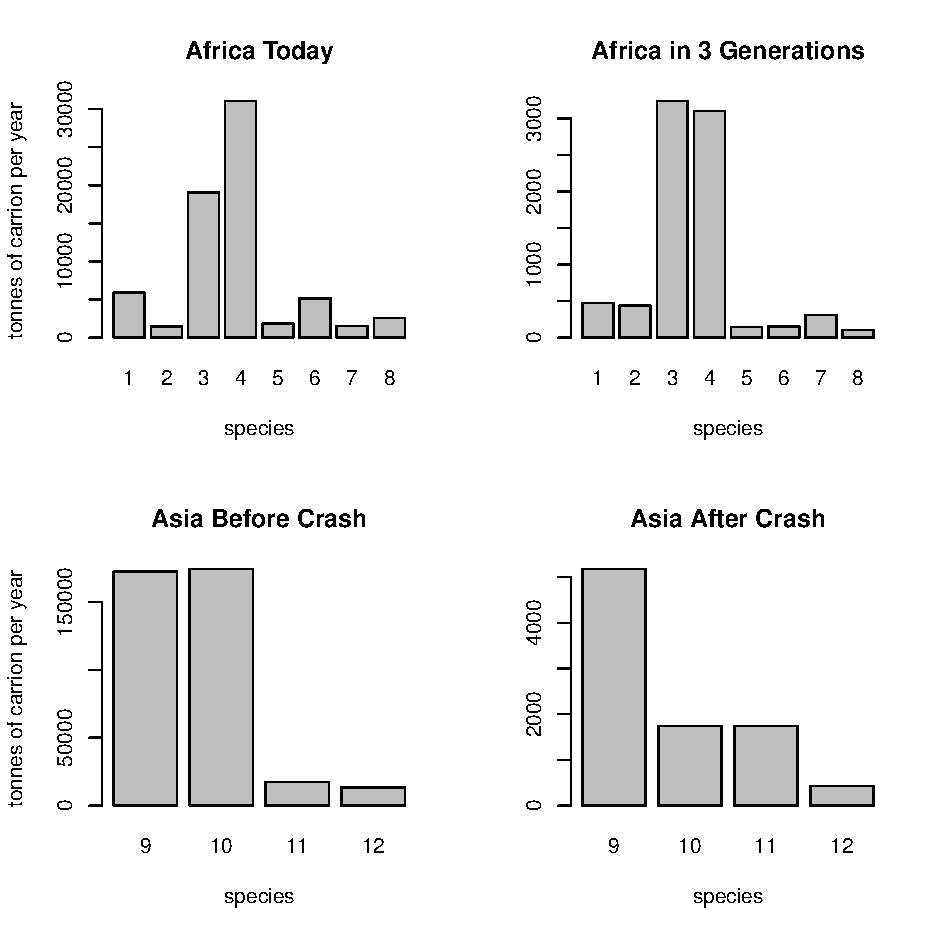
\includegraphics[keepaspectratio,totalheight=0.7\textheight]{VultureFood.pdf}
\caption{Food left behind in the case of African and Asian vulture declines}
\label{Vultures Asia and Africa food}
\end{figure}

%---------------------------------------------
%
%       DISCUSSION
%
%---------------------------------------------

\section{Discussion}
Difference in hyenas and vultures. Implications for the future. 

%Biology letters various stuff
\section{Ethics statement}
N/A
\section{Data accessibility statement}
All data and analysis code is available on GitHub (\url{https://github.com/kanead}).
\section{Authors' Contributions}
A.K. and A.J conceived and designed the experiments. A.K. performed the experiments and analysed the data. A.K. and A.J. contributed to the writing of the manuscript. All authors approved the final version of the manuscript.
\section{Competing Interests}
We have no competing interests.
\section{Acknowledgments}
We thank Thomas Guillerme.
\section{Funding statement}
This work was funded by a Trinity College Dublin Teaching Studentship.

\bibliographystyle{vancouver}
\bibliography{References}

%END
\end{document}
